\section{緒言}%===========================
エアシリンダは生産現場などに多く使われている.しかし,長いストロークを持ちつつも,コンパクトに使用するような場合には適合しない.よって,十分にストロークがありつつも,設置しやすい直動アクチュエータが求められている.
\par
そこで,曲げられるエアシリンダを開発する.本研究では曲げられるエアシリンダを"エアシリンダ型人工筋肉"と呼ぶ.エアシリンダ型人工筋肉は柔らかい素材で構成されている.そのため,曲がった状態で配置・動作し,高ストロークを有しつつもコンパクトに設置することができる.

しかし,エアシリンダ型人工筋肉は曲がった状態において,シリンダとロッドが接触する現象が起こる.本稿では,1つ目の内容として,シリンダを環状に巻き付けた状態における理論出力を導出し,実験値と比較する.
\par
2つ目の内容として,エアシリンダ型人工筋肉を機械要素として使用する際の制御特性について確認を行う.エアシリンダ型人工筋肉を揺動アームの機械要素とし,アームの角度制御とアーム先端のコンプライアンス制御を行い,制御性について評価を行う.
これら3つの内容を踏まえて,エアシリンダ型人工筋肉及びエアシリンダ型人工筋肉が機械要素としてどのように取り扱うかを確認する.
% エアシリンダ型人工筋肉の基礎特性,細径エアシリンダを束ねた構造の基礎特性とステップ応答性,曲がった状態のエアシリンダの理論と実験,エアシリンダ型人工筋肉を取り付けた揺動アームの位置制御とコンプライアンス制御

% 1.エアシリンダ型人工筋肉の開発
% 2.基礎特性の測定
% 3.曲がったエアシリンダ型人工筋肉の出力の理論化と実験値の比較
% 4.揺動アームの制御

\begin{figure}[t]
  \centering
  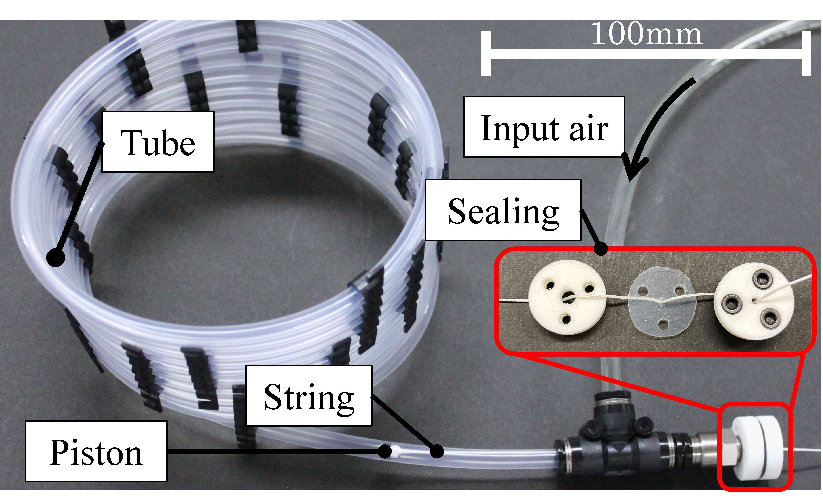
\includegraphics[width=85mm]{_pdf/細径柔軟エアシリンダ-1本.pdf}
  \caption{Air cylinder type artificial muscle}
  \label{Air cylinder type artificial muscle}
\end{figure}

\section{エアシリンダ型人工筋肉の開発}%-----------
\subsection{構造}%-----------
本研究で取り扱うエアシリンダ型人工筋肉とフィッティグの構造を図\ref{Air cylinder type artificial muscle}に示す.シリンダ部分は柔軟チューブ(ニチアス株式会社,材質:ナフロン\textregistered,内外径:$\SI{5}{mm}$, $\SI{6}{mm}$,最小曲げ半径:$\SI{35}{mm}$)である.ロッド部分は紐(ハヤミ工産株式会社,材質:イザナス®,線形:$\SI{0.60}{mm}$,破断強度:$\SI{360}{N}$,破断伸度:$\SI{5.5}{N}$)である.ピストンは2枚のフッ素ゴムリングを2枚のPLA樹脂部品で挟み込む構造である.シール部はゴムシート(材質:NBR,厚さ:1 mm,硬度:70 °(タイプA))である.ゴムシートに穴をあけてロッドを通している.ロッドを通したゴムシートを2つのプラスチック部品をボルトにより挟み込む.

\section{基礎特性の測定}%-----------
エアシリンダ型人工筋肉の各部品間には抵抗力が存在する.1つ目は,シール部と紐の接触による摩擦抵抗$D_s$である.2つ目は,チューブとピストンの接触による摩擦抵抗$D_\mathrm{p}$である.3つ目は,チューブと紐の接触による摩擦抵抗$D_\mathrm{t}$である.抵抗$D_\mathrm{s}$,$D_\mathrm{p}$は印加圧力によって変化すると考えられる.抵抗$D_\mathrm{t}$はチューブと紐の接触角$\theta$によって変化すると考えられる.よって,これら3つの抵抗力$D_\mathrm{s}(P_\mathrm{in})$,$D_\mathrm{p}(P_\mathrm{in})$,$D_\mathrm{t}(\theta)$を実験により測定した.以下に各抵抗$D_\mathrm{s}(P_\mathrm{in})$,$D_\mathrm{p}(P_\mathrm{in})$,$D_\mathrm{t}(\theta)$の実験式を示す.
\begin{align}
  D_\mathrm{s} & = \num{-4.0e-4}P_\mathrm{in} + \num{5.6e-4} \\
  D_\mathrm{p} & = \num{2.1e-3}P_\mathrm{in} + \num{4.0e-4}  \\
  D_\mathrm{t} & = 0.981e^{0.090\theta}
\end{align}


\section{環状に曲がったエアシリンダ型人工筋肉の理論出力}%-----------
\subsection{理論出力の導出}%-----------

\subsection{理論値と実験値の比較}%-----------

\section{エアシリンダ型人工筋肉を用いた揺動アームの開発}%-----------
\subsection{揺動アームの構造}
\subsection{揺動アームの角度制御}

\section{結言}%-----------